\mbox{$\displaystyle -\,\frac{1}{2}$\,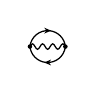
\begin{tikzpicture}[x=0.450cm, y=0.450cm, line width=0.450pt, baseline={([yshift=-0.6ex]0,0)}]
  \draw (0.500,0.000) arc[start angle=353.974, end angle=186.026, radius=0.503];
  \fill (-0.097,-0.450) -- (0.097,-0.533) -- (0.034,-0.450) -- (0.097,-0.367) -- cycle;
  \draw plot[smooth, tension=0.7] coordinates {(-0.500,0.000) (-0.464,0.055) (-0.429,0.077) (-0.393,0.055) (-0.357,0.000) (-0.321,-0.055) (-0.286,-0.077) (-0.250,-0.055) (-0.214,0.000) (-0.179,0.055) (-0.143,0.077) (-0.107,0.055) (-0.071,0.000) (-0.036,-0.055) (0.000,-0.077) (0.036,-0.055) (0.071,0.000) (0.107,0.055) (0.143,0.077) (0.179,0.055) (0.214,0.000) (0.250,-0.055) (0.286,-0.077) (0.321,-0.055) (0.357,0.000) (0.393,0.055) (0.429,0.077) (0.464,0.055) (0.500,0.000)};
  \draw (-0.500,0.000) arc[start angle=173.974, end angle=6.026, radius=0.503];
  \fill (0.097,0.450) -- (-0.097,0.533) -- (-0.034,0.450) -- (-0.097,0.367) -- cycle;
  \fill (-0.500,0.000) circle (0.064);
  \fill (0.500,0.000) circle (0.064);
\end{tikzpicture}}
\diagramgap
\mbox{$\displaystyle +\,\frac{1}{2}$\,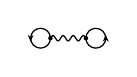
\begin{tikzpicture}[x=0.450cm, y=0.450cm, line width=0.450pt, baseline={([yshift=-0.6ex]0,0)}]
  \draw plot[smooth, tension=0.7] coordinates {(-0.500,0.000) (-0.464,0.055) (-0.429,0.077) (-0.393,0.055) (-0.357,0.000) (-0.321,-0.055) (-0.286,-0.077) (-0.250,-0.055) (-0.214,0.000) (-0.179,0.055) (-0.143,0.077) (-0.107,0.055) (-0.071,0.000) (-0.036,-0.055) (0.000,-0.077) (0.036,-0.055) (0.071,0.000) (0.107,0.055) (0.143,0.077) (0.179,0.055) (0.214,0.000) (0.250,-0.055) (0.286,-0.077) (0.321,-0.055) (0.357,0.000) (0.393,0.055) (0.429,0.077) (0.464,0.055) (0.500,0.000)};
  \draw (-0.500,0.000) arc[start angle=0.000, end angle=360.000, radius=0.280];
  \fill (-1.060,-0.097) -- (-0.977,0.097) -- (-1.060,0.034) -- (-1.143,0.097) -- cycle;
  \draw (0.500,0.000) arc[start angle=180.000, end angle=540.000, radius=0.280];
  \fill (1.060,0.097) -- (0.977,-0.097) -- (1.060,-0.034) -- (1.143,-0.097) -- cycle;
  \fill (-0.500,0.000) circle (0.064);
  \fill (0.500,0.000) circle (0.064);
\end{tikzpicture}}
\diagramgap
\mbox{$\displaystyle -\,$\,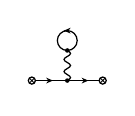
\begin{tikzpicture}[x=0.450cm, y=0.450cm, line width=0.450pt, baseline={([yshift=-0.6ex]0,0)}]
  \draw (0.000,0.000) -- (1.000,0.000);
  \fill (0.597,0.000) -- (0.403,0.083) -- (0.466,0.000) -- (0.403,-0.083) -- cycle;
  \draw (-1.000,0.000) -- (0.000,0.000);
  \fill (-0.403,0.000) -- (-0.597,0.083) -- (-0.534,0.000) -- (-0.597,-0.083) -- cycle;
  \draw plot[smooth, tension=0.7] coordinates {(0.000,0.850) (0.065,0.808) (0.092,0.765) (0.065,0.722) (0.000,0.680) (-0.065,0.638) (-0.092,0.595) (-0.065,0.552) (0.000,0.510) (0.065,0.467) (0.092,0.425) (0.065,0.382) (0.000,0.340) (-0.065,0.298) (-0.092,0.255) (-0.065,0.213) (0.000,0.170) (0.065,0.127) (0.092,0.085) (0.065,0.042) (0.000,0.000)};
  \draw (0.000,0.850) arc[start angle=270.000, end angle=630.000, radius=0.280];
  \fill (-0.097,1.410) -- (0.097,1.327) -- (0.034,1.410) -- (0.097,1.493) -- cycle;
  \draw[fill=white] (-1.000,0.000) circle (0.100);
  \draw[line width=0.320pt] (-0.930,0.070) -- (-1.070,-0.070) (-0.930,-0.070) -- (-1.070,0.070);
  \draw[fill=white] (1.000,0.000) circle (0.100);
  \draw[line width=0.320pt] (1.070,0.070) -- (0.930,-0.070) (1.070,-0.070) -- (0.930,0.070);
  \fill (0.000,0.850) circle (0.064);
  \fill (0.000,0.000) circle (0.064);
\end{tikzpicture}}
\diagramgap
\mbox{$\displaystyle +\,$\,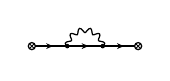
\begin{tikzpicture}[x=0.450cm, y=0.450cm, line width=0.450pt, baseline={([yshift=-0.6ex]0,0)}]
  \draw (0.500,0.000) -- (1.500,0.000);
  \fill (1.097,0.000) -- (0.903,0.083) -- (0.966,0.000) -- (0.903,-0.083) -- cycle;
  \draw (-1.500,0.000) -- (-0.500,0.000);
  \fill (-0.903,0.000) -- (-1.097,0.083) -- (-1.034,0.000) -- (-1.097,-0.083) -- cycle;
  \draw (-0.500,0.000) -- (0.500,0.000);
  \fill (0.097,0.000) -- (-0.097,0.083) -- (-0.034,0.000) -- (-0.097,-0.083) -- cycle;
  \draw plot[smooth, tension=0.7] coordinates {(-0.500,0.000) (-0.544,0.042) (-0.556,0.082) (-0.527,0.113) (-0.468,0.130) (-0.411,0.140) (-0.379,0.157) (-0.381,0.193) (-0.404,0.247) (-0.421,0.305) (-0.410,0.346) (-0.369,0.358) (-0.311,0.342) (-0.256,0.322) (-0.220,0.320) (-0.204,0.352) (-0.196,0.410) (-0.181,0.469) (-0.151,0.499) (-0.110,0.488) (-0.067,0.446) (-0.030,0.400) (0.000,0.380) (0.030,0.400) (0.067,0.446) (0.110,0.488) (0.151,0.499) (0.181,0.469) (0.196,0.410) (0.204,0.352) (0.220,0.320) (0.256,0.322) (0.311,0.342) (0.369,0.358) (0.410,0.346) (0.421,0.305) (0.404,0.247) (0.381,0.193) (0.379,0.157) (0.411,0.140) (0.468,0.130) (0.527,0.113) (0.556,0.082) (0.544,0.042) (0.500,0.000)};
  \draw[fill=white] (-1.500,0.000) circle (0.100);
  \draw[line width=0.320pt] (-1.430,0.070) -- (-1.570,-0.070) (-1.430,-0.070) -- (-1.570,0.070);
  \draw[fill=white] (1.500,0.000) circle (0.100);
  \draw[line width=0.320pt] (1.570,0.070) -- (1.430,-0.070) (1.570,-0.070) -- (1.430,0.070);
  \fill (-0.500,0.000) circle (0.064);
  \fill (0.500,0.000) circle (0.064);
\end{tikzpicture}}
\diagramgap
\mbox{$\displaystyle -\,\frac{1}{2}$\,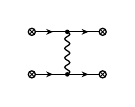
\begin{tikzpicture}[x=0.450cm, y=0.450cm, line width=0.450pt, baseline={([yshift=-0.6ex]0,0)}]
  \draw (0.000,0.600) -- (1.000,0.600);
  \fill (0.597,0.600) -- (0.403,0.683) -- (0.466,0.600) -- (0.403,0.517) -- cycle;
  \draw (0.000,-0.600) -- (1.000,-0.600);
  \fill (0.597,-0.600) -- (0.403,-0.517) -- (0.466,-0.600) -- (0.403,-0.683) -- cycle;
  \draw (-1.000,0.600) -- (0.000,0.600);
  \fill (-0.403,0.600) -- (-0.597,0.683) -- (-0.534,0.600) -- (-0.597,0.517) -- cycle;
  \draw (-1.000,-0.600) -- (0.000,-0.600);
  \fill (-0.403,-0.600) -- (-0.597,-0.517) -- (-0.534,-0.600) -- (-0.597,-0.683) -- cycle;
  \draw plot[smooth, tension=0.7] coordinates {(0.000,0.600) (0.051,0.567) (0.072,0.533) (0.051,0.500) (0.000,0.467) (-0.051,0.433) (-0.072,0.400) (-0.051,0.367) (0.000,0.333) (0.051,0.300) (0.072,0.267) (0.051,0.233) (0.000,0.200) (-0.051,0.167) (-0.072,0.133) (-0.051,0.100) (0.000,0.067) (0.051,0.033) (0.072,0.000) (0.051,-0.033) (0.000,-0.067) (-0.051,-0.100) (-0.072,-0.133) (-0.051,-0.167) (0.000,-0.200) (0.051,-0.233) (0.072,-0.267) (0.051,-0.300) (0.000,-0.333) (-0.051,-0.367) (-0.072,-0.400) (-0.051,-0.433) (0.000,-0.467) (0.051,-0.500) (0.072,-0.533) (0.051,-0.567) (0.000,-0.600)};
  \draw[fill=white] (-1.000,0.600) circle (0.100);
  \draw[line width=0.320pt] (-0.930,0.670) -- (-1.070,0.530) (-0.930,0.530) -- (-1.070,0.670);
  \draw[fill=white] (-1.000,-0.600) circle (0.100);
  \draw[line width=0.320pt] (-0.930,-0.530) -- (-1.070,-0.670) (-0.930,-0.670) -- (-1.070,-0.530);
  \draw[fill=white] (1.000,0.600) circle (0.100);
  \draw[line width=0.320pt] (1.070,0.670) -- (0.930,0.530) (1.070,0.530) -- (0.930,0.670);
  \draw[fill=white] (1.000,-0.600) circle (0.100);
  \draw[line width=0.320pt] (1.070,-0.530) -- (0.930,-0.670) (1.070,-0.670) -- (0.930,-0.530);
  \fill (0.000,0.600) circle (0.064);
  \fill (0.000,-0.600) circle (0.064);
\end{tikzpicture}}
